% /*
%  * This file is part of OpenModelica.
%  *
%  * Copyright (c) 1998-2011, Linköpings University,
%  * Department of Computer and Information Science,
%  * SE-58183 Linköping, Sweden.
%  *
%  * All rights reserved.
%  *
%  * THIS PROGRAM IS PROVIDED UNDER THE TERMS OF THIS OSMC PUBLIC
%  * LICENSE (OSMC-PL). ANY USE, REPRODUCTION OR DISTRIBUTION OF
%  * THIS PROGRAM CONSTITUTES RECIPIENT'S ACCEPTANCE OF THE OSMC
%  * PUBLIC LICENSE.
%  *
%  * The OpenModelica software and the Open Source Modelica
%  * Consortium (OSMC) Public License (OSMC-PL) are obtained
%  * from Linköpings University, either from the above address,
%  * from the URL: http://www.ida.liu.se/projects/OpenModelica
%  * and in the OpenModelica distribution.
%  *
%  * This program is distributed  WITHOUT ANY WARRANTY; without
%  * even the implied warranty of  MERCHANTABILITY or FITNESS
%  * FOR A PARTICULAR PURPOSE, EXCEPT AS EXPRESSLY SET FORTH
%  * IN THE BY RECIPIENT SELECTED SUBSIDIARY LICENSE CONDITIONS
%  * OF OSMC-PL.
%  *
%  * See the full OSMC Public License conditions for more details.
%  *
%  */

% This is the main file for a simulation runtime draft in OpenModelica
%
% draft.tex
%    $LastChangedRevision: 1 $ $LastChangedDate: 2011-10-25  $
%

\documentclass
[
%draft,
12pt
]{scrartcl}

\usepackage[bookmarks,hidelinks,breaklinks]{hyperref}

% Add some further packages
\usepackage{amsmath, amssymb, amsfonts, amsthm, amsbsy}
\usepackage{url}               % Handling of URL strings.

\usepackage{graphicx, color}
% uncomment according to your operating system:
% ------------------------------------------------
%\usepackage[latin1]{inputenc}    %% european characters can be used (Windows,
%old Linux)
\usepackage[utf8]{inputenc}     %% european characters can be used (Linux)
%\usepackage[applemac]{inputenc} %% european characters can be used (Mac OS)
% ------------------------------------------------
\usepackage[T1]{fontenc}   %% get hyphenation and accented letters right
%\usepackage{mathptmx}      %% use fitting times fonts also in formulas
% do not change these lines:
\pagestyle{empty}                %% no page numbers!

%****************** Modelica Listings **********************************
\usepackage{listings}
%% listings-modelica.cfg
%% Copyright 2014 Martin Sjoelund, Dietmar Winkler
%
% This work may be distributed and/or modified under the
% conditions of the LaTeX Project Public License, either version 1.3
% of this license or (at your option) any later version.
% The latest version of this license is in
%   http://www.latex-project.org/lppl.txt
% and version 1.3 or later is part of all distributions of LaTeX
% version 2005/12/01 or later.
%
% This work has the LPPL maintenance status `maintained'.
%
% The Current Maintainer of this work is Dietmar Winkler
%
% Code repository https://github.com/modelica-tools/listings-modelica
%
% This work consists of the file listings-modelica.cfg

\lstdefinelanguage{modelica}
{
  morekeywords=[1]{
    algorithm,and,annotation,as,assert,block,break,case,class,connect,connector,
    constant,constrainedby,der,discrete,each,else,elseif,elsewhen,encapsulated,
    end,enumeration,equality,equation,expandable,extends,external,failure,final,
    flow,for,function,guard,if,import,in,initial,inner,input,List,local,loop,
    match,matchcontinue,model,not,operator,Option,or,outer,output,package,parameter,
    partial,protected,public,record,redeclare,replaceable,return,stream,
    subtypeof,then,Tuple,type,uniontype,when,while},
  morekeywords=[2]{true, false},
  % Do not make true,false keywords because fn(true,x, false ) shows up as fn(true,x, *false*)
  sensitive=true,
  comment=[l]//,
  morecomment=[s]{/*}{*/},
  alsodigit={.,-},
  morestring=[b]',
  morestring=[b]",
}[keywords,comments,strings]

\definecolor{keywordcolor1}{rgb}{0,0,.4}
\definecolor{keywordcolor2}{rgb}{.90,0,0}
\definecolor{stringcolor}{rgb}{0.133,0.545,0.133}
% \definecolor{listingbgcolor}{rgb}{0.95,0.95,0.95}

\lstset{
  breaklines=true,
  language=modelica,
  basicstyle=\ttfamily,
  keywordstyle=[1]\color{keywordcolor1}\bfseries,
  keywordstyle=[2]\color{keywordcolor2},
  stringstyle=\color{stringcolor},
%  backgroundcolor=\color{listingbgcolor},
  framexleftmargin=5pt,
  xleftmargin=5pt,
  xrightmargin=5pt,
  showstringspaces=false,
}

\lstset{breaklines=true,label=}
% \lstset{basicstyle=\ttfamily}

\newcommand{\code}[1]{\texttt{\hyphenchar%
\font45%
\sloppy%
\fontdimen2\font=0.4em%
\fontdimen3\font=0.2em%
\fontdimen4\font=0.1em%
\fontdimen7\font=0.1em%
 #1}}


\lstset{language=modelica}

\usepackage{bibliography/biblatex}

% begin the document
\begin{document}
\thispagestyle{empty}
\title{\textbf{
Draft for a simulation runtime in OpenModelica
}}
% contributers, please add here your name if you have
% contribute to this draft.
\author{Willi Braun}
\date{\today} % <--- leave date empty
\maketitle\thispagestyle{empty} %% <-- you need this for the first page

\abstract{
This draft describes the current state of the OpenModelica run-time and the
requirements of improvements for the current c-run-time. }

\emph{Keywords: Simulation, c-run-time, solver, OpenModelica}

% /*
%  * This file is part of OpenModelica.
%  *
%  * Copyright (c) 1998-2011, Linköpings University,
%  * Department of Computer and Information Science,
%  * SE-58183 Linköping, Sweden.
%  *
%  * All rights reserved.
%  *
%  * THIS PROGRAM IS PROVIDED UNDER THE TERMS OF THIS OSMC PUBLIC
%  * LICENSE (OSMC-PL). ANY USE, REPRODUCTION OR DISTRIBUTION OF
%  * THIS PROGRAM CONSTITUTES RECIPIENT'S ACCEPTANCE OF THE OSMC
%  * PUBLIC LICENSE.
%  *
%  * The OpenModelica software and the Open Source Modelica
%  * Consortium (OSMC) Public License (OSMC-PL) are obtained
%  * from Linköpings University, either from the above address,
%  * from the URL: http://www.ida.liu.se/projects/OpenModelica
%  * and in the OpenModelica distribution.
%  *
%  * This program is distributed  WITHOUT ANY WARRANTY; without
%  * even the implied warranty of  MERCHANTABILITY or FITNESS
%  * FOR A PARTICULAR PURPOSE, EXCEPT AS EXPRESSLY SET FORTH
%  * IN THE BY RECIPIENT SELECTED SUBSIDIARY LICENSE CONDITIONS
%  * OF OSMC-PL.
%  *
%  * See the full OSMC Public License conditions for more details.
%  *
%  */

% This is the main file for a simulation runtime draft in OpenModelica
%
% content.tex
%    $LastChangedRevision: 1 $ $LastChangedDate: 2011-11-06  $
%

\section{Introduction}\label{sec:intro}

This draft summarizes all tasks which are needed to be done in the simulation
run-time for the modeling and simulation environment OpenModelica. The
simulation run-time is a library that is used with the generated model code to
be able to execute a simulation of the library. For the OMC exist several
run-time libraries and therefore the generated model code is different each
library.

\begin{itemize}
\item c-runtime
\item cpp-runtime
\item adevs-runtime
\item csharp-runtime
\end{itemize}

This draft is concerning the c-run-time. This library has grown over the
last few years. The historical growth is one reason for a weak structure.
Therefor the c-run-time will be reimplemented during the OpenModelica Developer
week in November 2011.

Further, this draft wants to setup a clear structure for the current tasks,
also with respect to future tasks.

The c-run-time is used for the following jobs:
\begin{itemize}
  \item Simulation of a generated model.
  \item FMI Export uses functions of the simulation run-time\cite{openmodelica.org:doc-extra:fmi1.0}.
  \item Interactive Simulation
  \item \ldots
\end{itemize}

Therefore, section \ref{sec:requirements} will state and describe all
requirements on a simulation run-time. In the next section \ref{sec:goals} the
goals for the redesign will be summarized.


\section{Requirements}\label{sec:requirements}

The main purpose of the simulation run-time is to calculate the simulation of a
translated model. In addition, there are some further tasks that are solved by
using functions of the simulation run-time (e.g. FMI, interactive simulation,
 etc.). The calculations that are needed to be done during the simulation
 process are specified in \ref{app:calculations}.

to be continued \ldots

\section{Goals for Redesign}\label{sec:goals}

\begin{itemize}
  \item Redesigning the usage of variables in the run-time. Separating static
  and dynamic variables (see \ref{sec:separetdata}).
  \item The reduction of the size of the generated model code and the size
  of every single function (see \ref{sec:ReduceSize}).
  \item Increasing the possibilities of debugging the solving process and
  provide better information for the users (see \ref{sec:debugging}).
  \item Fixing some issues in the current simulation run-time (see
  \ref{sec:currentsbugs}).
  \item Preparing the run-time for future tasks (see
  \ref{sec:runtimefuture}).
\end{itemize}

to be continued \ldots

\subsection{Separate static and dynamic variables}\label{sec:separetdata}

In the current c-run-time we have a \lstinline{struct sim_DATA} that
contains almost all data of a simulation model(see \ref{lst:simDATA}). This
should be separated in at least two parts. One part for dynamic variables and
one part for static variables. Further, we should create a new structure for all
simulation variables, that contain all information about it (e.g. current
value, start value, fixed-value, pre-value, max-min-values, etc.).

\begin{lstlisting}[label=lst:simDATA,caption={struct of the current sim\_DATA
from the current c\_runtim} ,language=C,commentstyle=\itshape] typedef struct
sim_DATA { /* this is the data structure for saving
  important data for this simulation.
  Each generated function has a DATA
  parameter which contains the data.
  An object for the data can be created using
  initializeDataStruc() function*/
  double* states;
  double* statesDerivatives;
  double* algebraics;
  double* parameters;
  double* inputVars;
  double* outputVars;
  double* helpVars, *helpVars_saved;
  double* initialResiduals;
  double* jacobianVars;
  /* True if the variable should be filtered */
  modelica_boolean* statesFilterOutput;
  modelica_boolean* statesDerivativesFilterOutput;
  modelica_boolean* algebraicsFilterOutput;
  modelica_boolean* aliasFilterOutput;
  /* Old values used for extrapolation */
  double* states_old, *states_old2, *states_saved, *states_start;
  double* statesDerivatives_old, *statesDerivatives_old2,
  *statesDerivatives_saved, *statesDerivatives_start;
   double* algebraics_old, *algebraics_old2,
   *algebraics_saved,*algebraics_start;
   double oldTime,oldTime2; double current_stepsize;
  /* Backup derivative for dassl */
  double* statesDerivativesBackup;
  double* statesBackup;
  char* initFixed; /* Fixed attribute for all variables and parameters */
  char* var_attr; /* Type attribute for all variables and parameters */
  int init; /* =1 during initialization, 0 otherwise. */
  int terminal; /* =1 at the end of the simulation, 0 otherwise. */
  void** extObjs; /* External objects */
  /* nStatesDerivatives == states */
  fortran_integer nStates,nAlgebraic,nParameters;
  long nInputVars,nOutputVars,nFunctions,nEquations,nProfileBlocks;
  fortran_integer nZeroCrossing/*NG*/;
  long nJacobianvars;
  long nRelations/*NREL*/;
  long nInitialResiduals/*NR*/;
  long nHelpVars/* NHELP */;
  /* extern char init_fixed[]; */
  DATA_STRING stringVariables;
  DATA_INT intVariables;
  DATA_BOOL boolVariables;
  DATA_REAL_ALIAS* realAlias;
  long nAlias;
  const char* modelName; /* For error messages */
  const char* modelFilePrefix; /* For filenames, input/output */
  /* to check if the model_init.xml match the model */
  const char* modelGUID;
  const struct omc_varInfo* statesNames;
  const struct omc_varInfo* stateDerivativesNames;
  const struct omc_varInfo* algebraicsNames;
  const struct omc_varInfo* parametersNames;
  const struct omc_varInfo* alias_names;
  const struct omc_varInfo* int_alg_names;
  const struct omc_varInfo* int_param_names;
  const struct omc_varInfo* int_alias_names;
  const struct omc_varInfo* bool_alg_names;
  const struct omc_varInfo* bool_param_names;
  const struct omc_varInfo* bool_alias_names;
  const struct omc_varInfo* string_alg_names;
  const struct omc_varInfo* string_param_names;
  const struct omc_varInfo* string_alias_names;
  const struct omc_varInfo* inputNames;
  const struct omc_varInfo* outputNames;
  const struct omc_varInfo* jacobian_names;
  const struct omc_functionInfo* functionNames;
  const struct omc_equationInfo* equationInfo;
  const int* equationInfo_reverse_prof_index;
  double startTime; /* the start time of the simulation */
  double timeValue; /* the time for the simulation */
  /* used in some generated function */
  /* this is not changed by initializeDataStruc */
  /* The last time value that has been emitted. */
  double lastEmittedTime;
  /* when != 0 force emit, set e.g.
  by newTime for equidistant output signal. */
  int forceEmit;
  /* An array containing the initial data of
  samples used in the sim */
  sample_raw_time* rawSampleExps;
  long nRawSamples;
  // The queue of sample time events to be processed.
  sample_time* sampleTimes; /* Warning: Not implemented yet!? */
  long curSampleTimeIx;
  long nSampleTimes;
} DATA;
\end{lstlisting}

All the variables in the listing \ref{lst:simDATA} and all other global
variables in the \verb+simulation_*.cpp+ files should categorised and separated
in of the categories in the figure \ref{fig:seperatedVariables}.
Therefore could be create a new file \verb+simulation_data.h+ that contains all
types.
$~~$\\


\begin{figure}[htb]
\begin{center}
  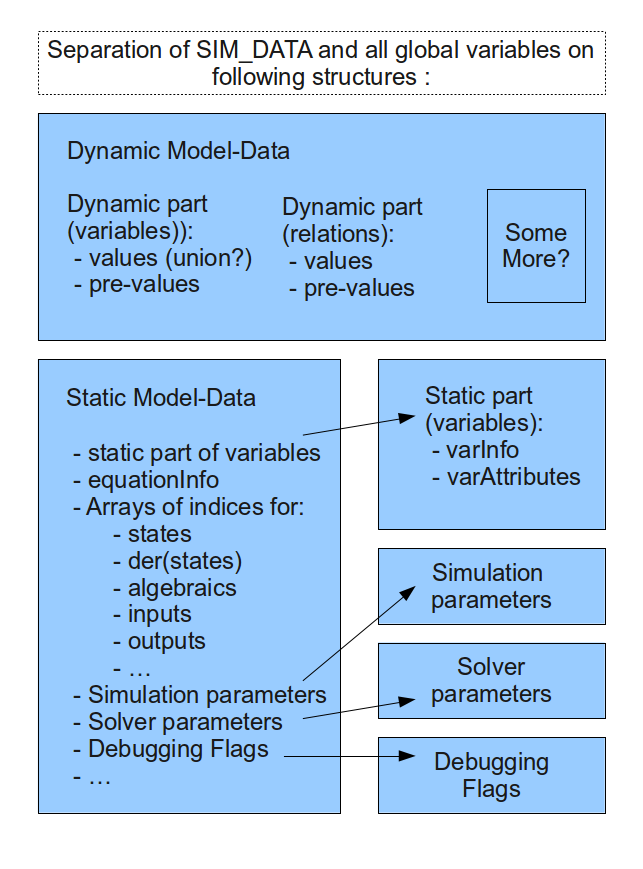
\includegraphics[width=0.5\textwidth]{SimulationRuntime/c/img/newSimDATA.png}
  \caption{Schematic separation of variables used in c-run-time.}
  \label{fig:seperatedVariables}
\end{center}
\end{figure}

\paragraph{Dynamic part}
\begin{description}
\item[dynamicVar] contains all values of the variables
that might be changed during the simulation. Hence we need to interpolate some
values during the simulation, we need also some old values stored here. For
handling events proper we need also save for every variable a pre-value.
\item[dynamicHelp] in the current implementation we save relations,
ZeroCrossings in \verb+helpvars+. So we should collect them all in central
structure that is organized similar to all other variables.
\item[More?]
\end{description}

\paragraph{Static part:}
\begin{description}
\item[staicVar] contains all static information about a variable of the
simulated model. The static information consists of varInfo and varAttributes.
\item[equationInfo] a structure defined in \verb+simulation_varinfo.h+.
\item[lookupVars] contains the indices for the categorised variables (states,
der(states), algebraics, etc.) of the dynamicVar array.
\item[SimData] contains all parameters to control the simulation process.
\item[SolverData] contains all parameters to setup the used solver.
\item[debugFlags] contains the flags for debugging the simulation.
\item[More?]
\end{description}

\subsubsection{implementation issues}

unions, ring buffer ???
to be continued in more detail \ldots


\subsection{Reducing the size of the generated model code and generated
functions}\label{sec:ReduceSize}

Currently, we generate almost every equation one time for ``functionODE'' and
``functionAlgebraics'' and a second time for ``functionDAE''. This could be
avoided by generating every equation or equation-block just one time and
creating one function with a parameter for the context in which this function
is going to be executed. There are two different context where an equation
can be executed: (1) during a continuous integration, where changing of
relations and discrete variables is forbidden. (2) during an event, where the
relations and discrete variables can be changed.
Thus the size of the generated model will be reduced all in all and also the
size of generated functions. Therefore this will result in a huge speed
up of the compile time of the ``gcc'' for bigger models.

to be continued in more detail \ldots

\subsection{Increasing the possibilities of debugging}\label{sec:debugging}

This subsection addresses the following two issues:
\begin{itemize}
  \item Providing better information about the solving process to the users.
  \item Creating possibilities for debugging the solving process from the
  point of view of a developer \cite{openmodelica.org:pop:sims:2007}.
\end{itemize}

to be continued \ldots

\subsection{The Requirements of the run-time in the
future}\label{sec:runtimefuture}

As some requirements in the future we could address the following issues:
\begin{itemize}
  \item Handling appropriate dynamic state selection.
  \item Handling varying structure problems.
  \item Preparing the run-time for parallelization of the simulation
  process.
 \item \ldots
\end{itemize}
This topics should be discussed further at the developer week.

to be continued \ldots

\subsection{Current unsolved issues in the run-time}\label{sec:currentsbugs}

In the current run-time there are also some issues, which aren't handled
appropriate right now or missing at all. They should also be addressed during
this redesign.
\begin{itemize}
  \item Algorithm sections should be initialized correctly. Therefore the start
  values of all variables are needed.
  \item Some Modelica statements are not supported appropriately.
  Following a first small list.
  \begin{description}
     \item[parameters] There is no separation of primary and secondary
     parameters. So that one could think to change secondary parameters in
     the init-file.
     \item[input varibales] There is no possibility to provide input variables
     by files.
     \item[Special Statements] \lstinline{assert()} and \lstinline{terminate()} are not handled
     appropriately. \\
     \item[initial()] In the current run-time the expression
     \lstinline{when not initial() then ... } is not handled appropriately.
     \item[] \ldots
   \end{description}
   \item \ldots
\end{itemize}

to be continued \ldots

\section{Overview of current c-runtime}

to be continued \ldots

% In this section is summarized which files are located in the current c-run-time.
%
% \begin{tabular}{ l l }
% base\_array.* & how base arrays are represented in C. \\
% boolean\_array.* & how arrays of booleans are represented in C. \\
% integer\_array.* & how arrays of integers are represented in C. \\
% real\_array.* & how arrays of reals are represented in C. \\
% string\_array.* & how arrays of strings are represented in C. \\
% index\_spec.c & keep track of dimension sizes of arrays. \\
% memory\_pool.c & memory allocation for local variables. \\
% read\_write.* & reading and writing of data to file. \\
% utility.* & utility functions \\
% modelica\_string.* & string functions
% \end{tabular}


%\section{Implementation issues}


\appendix
\section{Calculations during the simulation}\label{app:calculations}

Flat hybrid DAEs could represent continuous-time behavior and
discrete-time behavior. This is done mathematically by the equation
(\ref{eq:flat_dae_im}).

\begin{equation}\label{eq:flat_dae_im}
  F(  \underline{\dot x}(t),
  \underline{x}(t),
  \underline{u}(t),
  \underline{y}(t),
  \underline{q}(t_e),
  \underline{q_{pre}}(t_e),
  \underline{c}(t_e),
  \underline{p_{P}},
  \underline{p_{S}},
  \underline{s_0},
  t) = 0
\end{equation}

This implicit equation (\ref{eq:flat_dae_im}) is transformed to the explicit
representation of equation (\ref{eq:flat_dae_ex}) by block-lower-triangular
transformation.
\begin{equation}\label{eq:flat_dae_ex}
    %\underline{z} =
     \left(  \begin{array}{c}
         \underline{\dot x}(t) \\
         \underline{y}(t) \\
         \underline{q}(t_e)
       \end{array} \right) =
      \left( \begin{array}{c}
      \underline{f_s}(\underline{x}(t),
        \underline{u}(t),
        \underline{q_{pre}}(t_e),
        \underline{c}(t_e),
        \underline{p_{P}},
        \underline{p_{S}},
        \underline{s_0},
        t) \\
      \underline{f_a}(\underline{x}(t),
        \underline{u}(t),
        \underline{q_{pre}}(t_e),
        \underline{c}(t_e),
        \underline{p_{P}},
        \underline{p_{S}},
        \underline{s_0},
        t) \\
      \underline{f_q}(\underline{x}(t),
        \underline{u}(t),
        \underline{p},
        \underline{q_{pre}}(t_e),
        \underline{c}(t_e),
        \underline{p_{P}},
        \underline{p_{S}},
        \underline{s_0},
        t)
      \end{array} \right)
\end{equation}
From this explicit form all necessary calculations can be educed for the
simulation of the model. This is done by formulating the
continuous-time part, followed by the discrete-time part. Below are
summarized the notation used in the following equations:


\begin{itemize}
\item $\underline{\dot x}(t)$, the differentiated vector of state variables of
the model.
\item $\underline{x}(t)$, the vector of state variables of the model, i.e.,
variables of type \verb+Real+ that also appear differentiated, meaning that \verb+der()+ is
applied to them somewhere in the model.
\item $\underline{u}(t)$, a vector of input variables, i.e., not dependent on
other variables, of type \verb+Real+. They also belong to the set of algebraic
variables since they do not appear differentiated.
\item $\underline{y}(t)$, a vector of Modelica variables of type \verb+Real+
which do not fall into any other category.
\item $\underline{q}(t_e)$, a vector of discrete-time Modelica variables of type
discrete \verb+Real+, \verb+Boolean+, \verb+Integer+ or \verb+String+. These variables
change their value only at event instants, i.e., at points $t_e$ in time.
\item $\underline{q_{pre}}(t_e)$, the values of $q$ immediately before the
current event occurred, i.e., at time $t_e$.
\item $\underline{c}(t_e)$, a vector containing all \verb+Boolean+ condition
expressions evaluated at the most recent event at time $t_e$. This includes conditions from
all \verb+if+-equations and \verb+if+-statements and \verb+if+-expressions from
the original model as well as those generated during the conversion of \verb+when+-equations
and \verb+when+-statements.
\item $\underline{p_{P}} = {p1, p2, \ldots}$, a vector containing the Modelica
variables declared as \textbf{primary parameter} i.e., variables without any
time dependency and without a dependence on other parameters.
\item $\underline{p_{S}} = {p1, p2, \ldots}$, a vector containing the Modelica
variables declared as \textbf{secondary parameter} i.e., variables without any
time dependency, but with a dependence on other parameters.
\item $\underline{s_0} = {s1, s2, \ldots}$ all start values in the model.
\item $t$, the Modelica variable time, the independent variable of type
\verb+Real+ implicitly occurring in all Modelica models.
% \item $relation(v(t))$, a \verb+Boolean+ vector valued function containing the
% relevant elementary relational expressions from the model, excluding relations enclosed
% by \verb+noEvent()+. The argument $v(t) = {v1,v2,\ldots}$ is a vector
% containing all elements in the vectors $x(t)$, $\dot x(t)$, $u(t)$, $y(t)$,
% $q(t_e)$,$q_{pre}(t_e)$, $p$, $t$.
\end{itemize}

\subsection{Continuous Behavior}

The continuous behavior of hybrid DAEs can be formulated with the
following equations (\ref{eq:hybrid_con}).
\begin{equation} \label{eq:hybrid_con}
\left (    \begin{array}{c}
         \underline{\dot x}(t) \\
         \underline{y}(t)
       \end{array} \right) =
      \left( \begin{array}{c}
      \underline{f_s}(\underline{x}(t),
        \underline{u}(t),
        \underline{q_{pre}}(t_e),
        \underline{c}(t_e),
        \underline{p_{P}},
        \underline{p_{S}},
        \underline{s_0},
        t) \\
      \underline{f_a}(\underline{x}(t),
        \underline{u}(t),
        \underline{q_{pre}}(t_e),
        \underline{c}(t_e),
        \underline{p_{P}},
        \underline{p_{S}},
        \underline{s_0},
        t)
     \end{array} \right)
\end{equation}
The states $\underline{x}(t)$ are determined by an integration method, so that
they are assumed to be known as the vectors $\underline{u}(t)$ and
$\underline{p_{[P|S]}}$.
For discrete variables and the condition expressions $t_e$ is used instead of
$t$ to indicate that such variables may only change values at event points of
time and are kept constant in the continuous parts of the simulation.

Imported is also that all conditions $\underline{c}(t_e)$ are kept on there
current value for the whole continuous step. If the continuous step cause

\subsection{Discrete Behavior}

The discrete behavior is controlled by events. Events are triggered by the
event conditions $\underline{c}(t_e)$ and can appear at any time
as well as influence the system several times.

An event occurs when a condition of $\underline{c}(t_e)$ changes it's value at
time $t_e$ from \verb+false+ to \verb+true+ or the other way around.
This occurs if and only if for a sufficient small $\epsilon$, one condition in
$\underline{c}(t_e)$ is changed, for e.g. $\underline{c}(t_e - \epsilon)$ is
\verb+false+ and for $\underline{c}(t_e + \epsilon)$ is \verb+true+. When an event
occurs all caused changes in the system can be carried out. In addition, the
entire system must be determined by the function (\ref{eq:flat_dae_ex}) to
guarantee the synchronism of all equations. However, it is not enough to
determine only the discrete variables by the function $\underline{f_q}$ at
this point.

The problem to be solved here is the most accurate determination of the event
time $t_e$. For this conditions $\underline{c}(t_e)$ can be divided into three
groups.
\begin{enumerate}
  \item Conditions $\underline{c_k}(t_e)$, which also depend on continuous
  variables.
  \item Conditions $\underline{c_d}(t_e)$, that only depend on discrete
  variables.
  \item Conditions $\underline{c_{\text{noEvent}}}(t)$, are evaluated without
  resulting in an event.
\end{enumerate}

If the \verb+smooth+ operator applies to a condition in $\underline{c}(t_e)$
this condition can be categorized depending on the order of the integration
method by 1. or 3., respectively.

The second and third group of conditions are easy to handle, because if a
condition in $\underline{c}(t_e)$ only depends on discrete variables, then they
could only change at events and the conditions $\underline{c_d}(t_e)$ must be
tested only at events. The conditions $\underline{c_{\text{noEvent}}}(t)$
result logically in no events. Thus, the equations which depend on conditions
$\underline{c_{\text{noEvent}}}(t)$, will be determined during the continuous
integration at the output points. Hence the variables that are determined by
the function (\ref{eq:qnoevent}) should be treated appropriately, like
algebraic variables.
\begin{equation}\label{eq:qnoevent}
\underline{q_{\text{noEvent}}(t)} :=
g(\underline{x}(t_e), \underline{u}(t_e), \underline{q_{pre}}(t_e),
\underline{c_{\text{noEvent}}}(t_e), \underline{p} ,t)
\end{equation}

What remains is the group of conditions, that lead to state events. For this
group of conditions a time-consuming search has to be performed.  These
conditions have to be checked during the continuous solution as described in the
next section.

Additional, discontinuous changes can caused by the \verb+reinit()+ operator to
the continuous states $\underline{x}(t)$.
As for purely discrete conditions $\underline{c_d}(t_e)$ the \verb+reinit()+
operator can only be activated at event times $t_e$ . This new allocation to
the states could use the function (\ref{eq:reinit}).

\begin{equation}\label{eq:reinit}
\underline{x(t_e)} := \underline{f_x}(\underline{x}(t),\underline{\dot
x}(t), \underline{u}(t), \underline{q}(t_e), \underline{q_{pre}}(t_e),
\underline{c}(t_e), \underline{p} ,t)
\end{equation}


\subsection{Run-time Algorithm}

A general approach for the simulation of hybrid systems has been developed by
Cellier ( cf. \cite{openmodelica.org:doc-extra:cellier1979}). In the following a schematic
Flowchart (see fig. \ref{fig:ablaufdiagramm}) for the simulation is shown and
each step is described.

First of all the simulation must be initialized consistently. For that the
initial values are found with a simplex optimization method in OpenModelica
(cf. \cite{openmodelica.org:bachmann:modelica:2006}). By use of the initial conditions the initial values
for the entire system can be determined with the function
(\ref{eq:flat_dae_ex}). This will also execute all initial events at time
$t_0$.
%Further an initialization of the corresponding ZeroCrossing function to
%the fullfilled condition at time $t_0$ is needed, to know its direction.

\begin{figure}[htb]
\begin{center}
  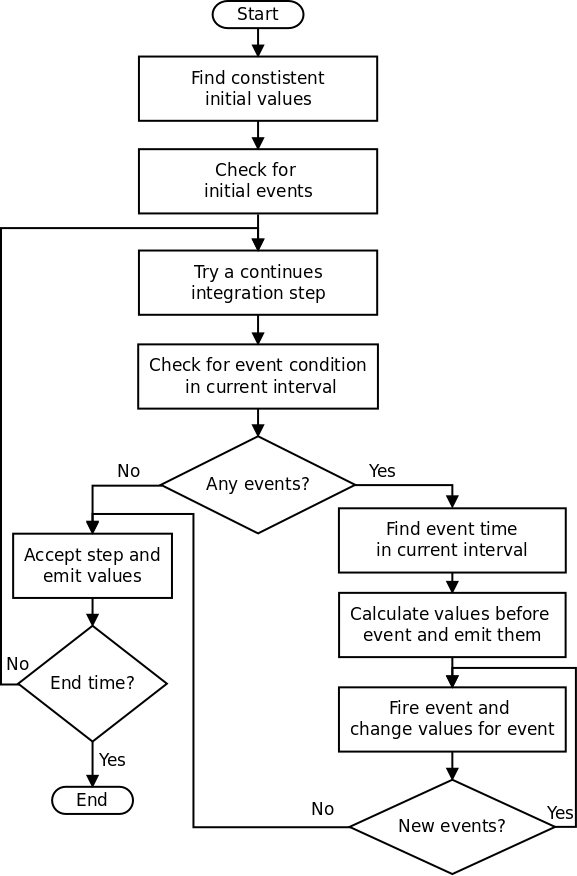
\includegraphics[width=0.47\textwidth]{SimulationRuntime/c/img/activitydiagramm.png}
  \caption{Schematic Flowchart for simulation hybrid models.}
  \label{fig:ablaufdiagramm}
\end{center}
\end{figure}

After the initialization the main simulation loop starts with the continuous
integration step that calculates the states $\underline{x}(t_{i+1})$.
With the new values of $\underline{x}(t_{i+1})$, the functions
$\underline{f_s}$ and $\underline{f_a}$ can be evaluated. Thus, the entire
continuous system is determined.

The continuous integration step is accepted if none of the
Zero-Crossing functions has a zero-crossing, i.e in $\underline{c}(t_{i+1})$ no
value has changed compared to $\underline{c}(t_i)$.
If no event has occurred the values can be saved and the next step can be performed.

However, if a value of $\underline{c}(t_{i+1})$ changes, an event occurred
within the interval $t_i$ and $ t_{i+1}$. Then the exact time $t_e$ has to be
detected. Therefore a root finding method is performed on the Zero-Crossing
functions of the corresponding conditions. If several Zero-Crossing functions
apply the first occurring root is chosen as the next event time $t_e$.

The next step is to prepare the treatment of an event by evaluating the system
just before an event at time $t_e - \epsilon $, and shortly after the event at $t_e +
\epsilon$. Current derivative-free root finding methods work under the
principle that the root is approximated through limits at the two sides,
so that the delivered root lies somewhere in the interval $[t_e - \epsilon;
t_e + \epsilon]$. Here $\epsilon$ is the tolerance level of the root finding
method. Thus the necessary information to treat the event are available after
the root is found.

The treatment of an event looks like that: The continuous part is evaluated at
the time just before the event $t_e - \epsilon$ and all values are saved to provide
them to the \verb+pre()+ operator. Then the entire system is evaluated
by the function (\ref{eq:flat_dae_ex}) at time $t_e + \epsilon$.
At this point the causing event is handled and now further caused events are
processed with the so-called Event-Iteration. Therefore the entire system
constantly is re-evaluated, as long as there exist discrete variables $q_j$
that satisfy \verb+pre(+$q_j$\verb+)+$\neq q_j$.  Only if for all discrete
variables \verb+pre(+$q_j$\verb+)+$ = q_j$ is fulfilled, the Event-Iteration
has reached a stable state and the next integration step can be performed.




\printbibliography[heading=bibintoc]

\end{document}
